
\subsubsection{Prerequisites}

\begin{itemize}
\item Reasonable quality beam tune. 
\item Beam current should be set  to $<10$ nA 
without exceeding a 5\% accidental rate of left-right coincidence.

\begin{itemize}
\item The optimal beam current is a function of beam energy.
More specific information may be available on the white board in the
counting house or in the run period specific documentation or web page. Regardless
of what currents are specified on the White board or this document,
the ratio $Left\otimes Right$ accidentals relative the true coincidence
rate should be kept below 5\%. It may be necessary to adjust the
HV on the Left and Right PMT's to achieve a low accidental rate, while
maintaining a reasonable true rate.
\end{itemize}
\item \textbf{Drift Chamber High Voltage OFF}
\item \textbf{SVT/MVT High Voltage OFF}
\item Harps are in the retracted position.
\end{itemize}

\subsubsection{Setup }

\begin{enumerate}
\item Notify MCC that you are about to do a M{\"o}ller run and \textbf{request
to take the beam to the tagger yoke beam dump} (they will need to take a beam
way and energize the tagger magnet). 
\item Wait for MCC to authorize change the BTA setting to ``photon
beam'' and also limits if necessary 
\item Ask MCC to turn orbit locks off and mask BOM and Downstream Halo
  Counters in FSD (if needed)
\item Once the tagger magnet is energized, request the beam current as specify for the given energy M{\o}ller measurements to be delivered, as measured by 2C21 nA BPM or SLM. Do
not use 2C24A since that BPM is located downstream of the M{\"o}ller setup
\item The following steps are all done from the EPICS terminal of one of \textbf{clonsl} PCs. The
M{\o}ller setup GUI is launched via the \textbf{Moller} button on the {}``beam\_screens'' GUI. 
%\latex{\ref{moller_epics}} on page\pageref{{moller_epics} } shows the
%M{\o}ller system GUI before the hardware has been set up. 

\begin{enumerate}
\item Make sure that the integration time for the asymmetry scalers is
set to 5 on the ``Asymmetry'' GUI. If it is not, use the slider to
set it to 5 (if the slider wont move, check ``IOC ACCESS'' on
``clas\_epics'' GUI on clonsl) 
 
\item Click the \emph{Configure Moller Hardware} button, near the top of
the GUI, Figure \ref{moller_epics_setup}. This will set off the following sequence of events:

\begin{enumerate}
\item SC HV Mainframes will be turned off.
\item EC HV Mainframes will be turned off.
\item Helmholtz Magnet will be energized in the Negative polarity.
\item M{\"o}ller Target will be positioned to the \emph{LEFT} target position.
\item M{\"o}ller Quadrupole magnets will be energized
\item EPICS DAQ will be started
\end{enumerate}
\item Watch the text at the top of the GUI for informational guidance.
\end{enumerate}
\end{enumerate}
%

\begin{figure}
\begin{center}
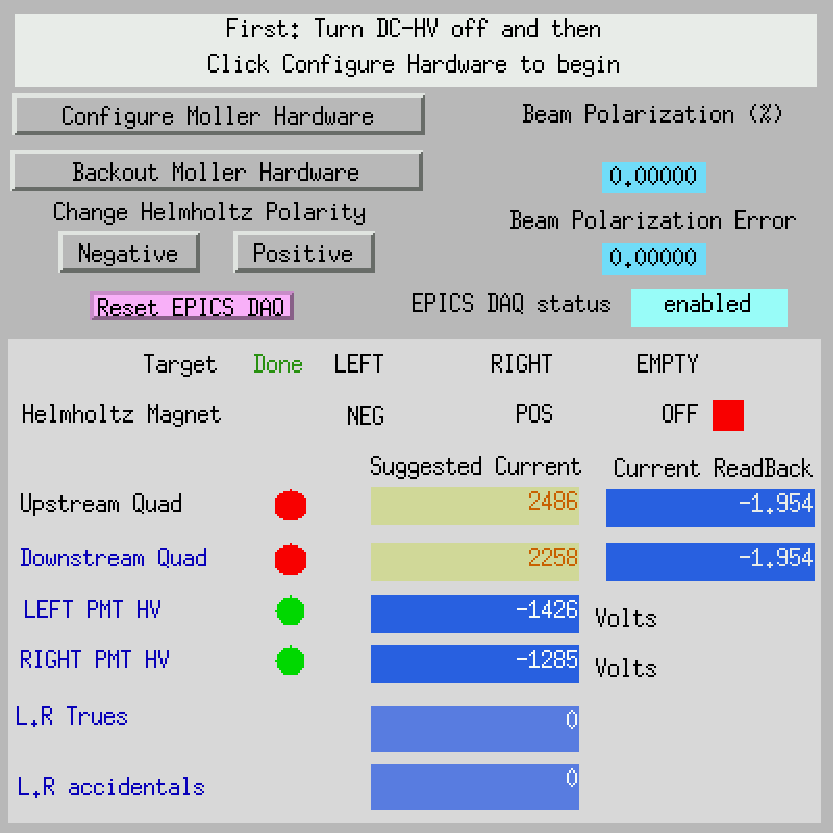
\includegraphics[width=0.75\textwidth]{moller_window.pdf}

\caption{The M{\"o}ller Epics screen of M{\"o}ller hardware
set up. \label{moller_epics_setup}}
\end{center}
\end{figure}


\subsubsection{Confirming the M{\"o}ller Hardware Configuration}

If the M{\"o}ller hardware is correctly set up you should observe
$L\bigodot R\, trues$ rate and the beam polarization should be posted
on the EPICS GUI. If no coincidence rate, or no beam polarization
on the GUI page the expert.


\subsubsection{Data Taking}

\begin{itemize}
\item Run is complete when the error on EPICS GUI on beam polarization is below
1.5\% absolute. Typicaly it takes about 30min to get required accuracy
\end{itemize}

\subsubsection{Close out\label{moller close out}}

When you finished the measurements:

Do not forget to make a log entry using ``Log Entry'' button on the GUI! 

Click the \emph{Backout Moller Hardware} button on the EPICS GUI to 
restore the hardware back to production running. 



Request that MCC take the beam away and \textbf{de-gauss the tagger
magnet.}

Once tagger magnet is degaussed, restore beam to Faraday Cup.

Turn on DC HV.


\subsubsection{Tips}

\begin{enumerate}
\item During a M{\"o}ller run the upstream PMTs labeled \char`\"{}up\char`\"{}
and \char`\"{}down\char`\"{} will get activated. The half life is
around 20 Minutes.~ MCC should ignore those PMTs for at least an
hour. 
\item MOLLER QUADS.~ At times the moller quads will not turn on.~ Using the moller expert screens controls you can try a few things to get
them on first try to click the \char`\"{}RESET\char`\"{} and \char`\"{}ON\char`\"{}
buttons.~ Then you could try to click the \char`\"{}OFF\char`\"{}
and then \char`\"{}ON\char`\"{} buttons.~ The readback value of the
current should be close to the entered set value.
\item Steering:~ Based on the beam tune, the moller quads may substantially
deflect the beam.~ A deflection of 5 mm has been observed.~ 
\item If the Moller PMT's do not come on try resetting them using the \char`\"{}clas\_epics\char`\"{}
program that is probably running on another monitor (maybe even the
clas10 monitor). Midway down theGUI you will see a button labeled
\char`\"{}tagger \& beam HV\char`\"{} under the caption \char`\"{}High
Voltage\char`\"{}. A window will open and you should select a button
on the first line (Group 1) under the column labeled Voltage/Current\char`\"{}.
This will spawn yet another window with a list of devices. The devices
labeled \char`\"{}BM\_MOLLER\_L\char`\"{} and \char`\"{}BM\_MOLLER\_R\char`\"{}
are the ones of interest to you. Use the \char`\"{}Dis\char`\"{} and
\char`\"{}Ena\char`\"{} buttons and the entry field \char`\"{}Input
V\char`\"{} to set the PMTs to -1551V for BM\_MOLLER\_L and -1410
for BM\_MOLLER\_R. (if this still fails page the Beamline person on
call).
\end{enumerate}

